\documentclass[10pt, a4paper, oneside]{article}

\usepackage[margin=1.25in]{geometry}
\usepackage[a-1b]{pdfx}
\usepackage[justification=centering]{caption}
\usepackage{amsthm}
\usepackage{amsmath}
\usepackage{amsfonts}
\usepackage[T1]{fontenc}
\usepackage{minted}
\usepackage[utf8]{inputenc}
\usepackage{graphicx}
\usepackage{subcaption}
\usepackage{fancyhdr} %abstract
\usepackage[italian]{babel}
\usepackage{listings}
\usepackage{todonotes}
\usepackage{color}
\usepackage{algorithm}
\usepackage{frontespizio}
\usepackage[noend]{algpseudocode}
\usepackage{tabularx}
\usepackage{hhline}
\usepackage[section]{placeins}

\usemintedstyle{autumn}

\RecustomVerbatimEnvironment{Verbatim}{BVerbatim}{}

\renewcommand{\figurename}{Listing}

\title{Rush Hour ASP solver}
\author{Fiorenzo Tittaferrante}







\begin{document}

\maketitle



\section{Introduzione}
\emph{Rush Hour} è un rompicapo logico che consiste nel spostare le varie auto per poter trovare una soluzione: come quando si è in macchina e bloccati nel traffico, l'obiettivo è uscire dall'ingorgo spostando i veicoli che impediscono all’automobile rossa di passare. \\

\noindent
Sul piano di gioco si posiziona l’auto rossa da far uscire dall’ingorgo e le auto del traffico. Le auto possono muoversi solamente verso l'alto o verso il basso, oppure a destra o a sinistra, in base alla direzione che ciascuna di esse possiede. Inoltre le auto hanno una dimensione di 2 oppure di 3 unità; in particolare l'auto rossa è lunga 2 unità.


\subsection{Convenzioni e scelte progettuali}\label{subsec:scelte_progettuali}
Il rompicapo è organizzato in una griglia $6\times6$ in cui ciascun punto è rappresentato da una coppia $(X,Y)$, dove la $X$ rappresenta la riga e la $Y$ la colonna. \\

\noindent
Stiamo affrontando un problema di pianificazione e il tempo svolge un ruolo fondamentale: ogni regola è descritta in primo luogo dal tempo $T$ in cui quell'azione accade. \\

\noindent
I nomi date alle auto sono: $r$ (\emph{red}) per l'auto rossa e $b1$, $b2$, $b3$ (e così via) per tutte le altre auto (di colore blu). Inoltre, per ogni auto è indicato l'orientamento di quest'ultima tramite \mint{prolog}|h| (\emph{horizontal}) e \mint{prolog}|v| (\emph{vertical}). \\
%I nomi date alle auto non sono casuali: corrispondono ciascuna ad un colore particolare ($r$ per \emph{red}, $k$ per \emph{black} e così via) e permettono ad uno script in python di poter distinguere e disegnare ciascuna auto, in ogni istante di tempo, nella propria posizione. Associato a ciascun auto è indicata l'orientamento di quest'ultima con \mint{prolog}|h| per \emph{horizontal} e \mint{prolog}|v| per \emph{vertical}. \\

\noindent % , a prescindere dalla sua lunghezza di 2 o 3.
La scelta progettuale più importante riguarda come strutturare un auto. Tra le varie possibilità analizzate vi sono:
\begin{itemize}
	\item[1] Strutturare l'auto con la sua dimensione e l'orientamento, per poi specificare successivamente la posizione.
	\item[2] Strutturare l'auto con la coordinata che rimane fissa ($X$ per le auto orizzontali e $Y$ per le auto verticali), seguita dalle altre coordinate che indica in quale riga o colonna si trovano i blocchi che compongono l'auto;
	\item[3] Strutturare l'auto come un insieme di blocchi creati separatamente: complesso da gestire.%, ma logicamente uniti.
\end{itemize}

\subsubsection{Versione 1}
La prima soluzione rende le auto indipendenti dalla propria lunghezza; è necessario semplicemente indicare una sola posizione, indicata dalla coppia $(X,Y)$ più piccola.


%problemi complessi: ad esempio lo spostamento in una delle possibili direzioni o la generazione di un'unica mossa, dovevano tener conto della lunghezza dell'auto per avere il numero totale di blocchetti da dover considerare e così via. \\
%La prima soluzione portava alla creazione di tanti blocchi singoli, che hanno lo stesso nome per rappresentare la stessa auto, ma con posizioni diverse: questa soluzione portava a problemi complessi, come ad esempio lo spostamento in una delle possibili direzioni o la generazione di un'unica mossa che sposti tutti i blocchetti contemporaneamente.

\subsubsection{Versione 2}
La seconda soluzione tiene traccia della posizione di ogni auto come se fosse un singolo blocco. Questo approccio è dipendente dalle dimensioni delle auto coinvolte nel puzzle, ovvero, per auto di dimensioni diverse è necessario creare dei predicati ad hoc per le posizioni e il loro aggiornamento, le azioni e la loro esecuzione.





% \subsubsection{Versione 3}
% La terza soluzione portava alla creazione di tanti blocchi singoli, che hanno lo stesso nome per rappresentare la stessa auto, ma con posizioni diverse. Questa soluzione portava ad ottenere un codice "macchinoso" e non di facile interpretazione. \\

% \noindent
% Sono state sviluppate le prime due versioni che verranno di seguito approfondite. \\


% \subsection{Esecuzione}
% Per eseguire (nel caso della prima versione) la risoluzione di un caso di test ci si può appoggiare ad uno script. \\

% \noindent
% È sufficiente eseguire \mint{shell}|sh 1-go| seguito dal nome del file del caso che si vuole risolvere, visualizzabili nella directory \emph{configuration}, e dalla lunghezza del tempo $l$. Lo script si occuperà di risolvere l'istanza scelta e nella directory \emph{images} produrrà una fotografia ad ogni istante di tempo della situazione di tutte le macchine ed una gif che riunisce tutti gli snapshot.\\

% \noindent
% Un esempio d'uso è il seguente:
% \begin{figure}[htp]
% \centering
% \begin{minted}{shell}
% sh 1-go sample01.lp 25
% \end{minted}
% \end{figure}



\newpage
\section{Implementazione versione 1}

\subsection{Premesse}
Il tempo in cui eseguire le azioni è fornito da linea di comando, invece la dimensione della griglia è fissa. Il fatto \mint{prolog}|moveTo| non ha un effettivo utilizzo, ma è usato per chiarezza del codice. Segue \mint{prolog}|orientation| che indica, come detto inizialmente, le \emph{\textbf{orientazioni}} possibili: \mint{prolog}|h| per \emph{horizontal} e \mint{prolog}|v| per \emph{vertical}. Il fatto \mint{prolog}|cars| rappresenta per semplicità il nome (o colore) di ciascuna auto. \\

\noindent
Iniziamo nel definire la parte estensionale del programma con i seguenti fatti.% con un semplice esempio.
\begin{figure}[htp]
\centering
\begin{minted}{prolog}
time(0..l).
grid(1..6,1..6).
moveTo(right; left; up; down).
orientation(h;v).
cars(r;b).
\end{minted}
\end{figure}


\noindent
\\L'auto è caratterizzata dal nome, dalla dimensione e dalla direzione.%, come detto precedentemente nella sezione \ref{subsec:scelte_progettuali}.
\begin{figure}[htp]
\centering
\begin{minted}{prolog}
car(r, 2, h).
car(b, 3, v).
\end{minted}
\label{code:car_defn}
\end{figure}

\noindent
\\Definito l'oggetto auto, si procede identificando la \emph{\textbf{posizione}} occupata indicandola tramite il valore dell'ascissa e dell'ordinata più piccola. Il punto nella griglia che si indica, quindi, è il punto iniziale dell'auto: per un auto orizzontale è il punto più a sinistra, per un auto verticale è il punto più in alto.
%oppure dall'alto verso il basso nel caso di orientamento verticale.
\begin{figure}[htp]
\centering
\begin{minted}{prolog}
position(0, r, 3, 1).
position(0, b, 2, 4).
\end{minted}
\label{code:position0}
\end{figure}

\noindent
\\Ciò che ci si aspetta quindi è di trovare, al tempo 0, il primo blocco dell'auto $r$ in $(3,1)$ (riga 3, colonna 1) ed essendo $r$ orizzontale e lunga 2, il secondo blocco è in posizione $(3,2)$. \\
Lo stesso ragionamento è valido per $b$ e l'immagine sottostante rappresenta la situazione descritta dai fatti appena visti.% \ref{code:car_defn} e \ref{code:position0} appena visti:
\begin{figure}[H]
  \centering
  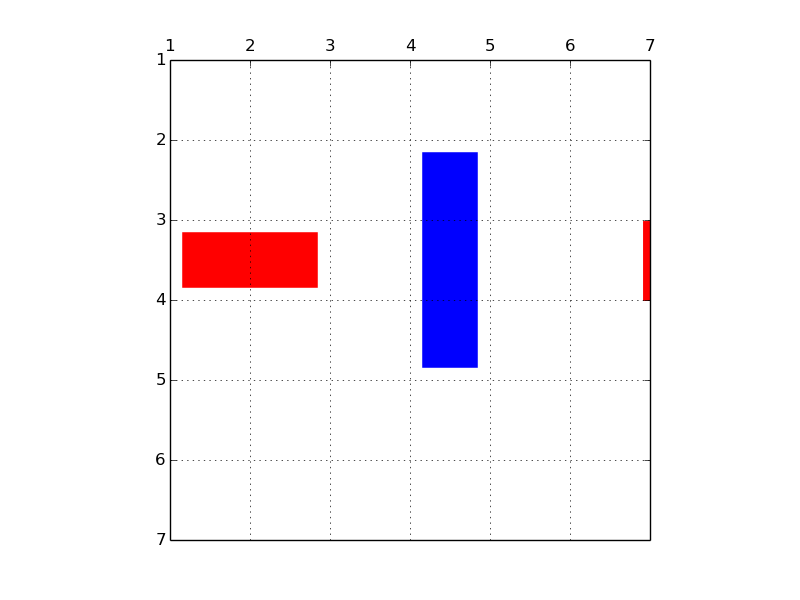
\includegraphics[width=0.4\textwidth]{images/0-example.PNG}
  \caption{Situazione iniziale al tempo 0}
  \label{fig:}
\end{figure}

























\newpage
\subsection{Occupazione}
È proprio grazie alla dimensione e all'orientamento dell'auto che è possibile capire tutte le posizioni nella griglia che l'auto occupa. \\

\noindent
La regola \mint{prolog}|busy(T, C, X, Y..Y+N-1)| calcola le \emph{\textbf{posizioni occupate}} da una determinata auto $C$ al tempo $T$ ed ha arità 4 con, rispettivamente:
\begin{itemize}
	\item Il tempo;
	\item Il nome dell'auto;
	\item La coordinata $X$ per le auto orizzontali;
	\item Un range di $Y$, per le auto orizzontali, per le posizioni di ciascun blocchetto che compongono l'auto lunga $N$.
\end{itemize}

\noindent
\\Di regole \mint{prolog}|busy| ve ne sono 2 per distinguere i casi di auto orizzontale e verticale e il corpo contiene \mint{prolog}|car(C, N, h)|, per ottenere che $C$ sia orizzontale e \mint{prolog}|position(T, C, X, Y)| per avere la posizione occupata da $C$ al tempo attuale $T$:

\begin{figure}[H]
\centering
\begin{minted}{prolog}
busy(T, C, X, Y..Y+N-1) :- time(T), T<l, 
                           position(T, C, X, Y), car(C, N, h).

busy(T, C, X..X+N-1, Y) :- time(T), T<l, 
                           position(T, C, X, Y), car(C, N, v).
\end{minted}
\label{code:busy}
\end{figure}


\noindent
\\Queste due regole graficamente generano la situazione raffigurata nell'immagine sottostante.
\begin{figure}[H]
  \centering
  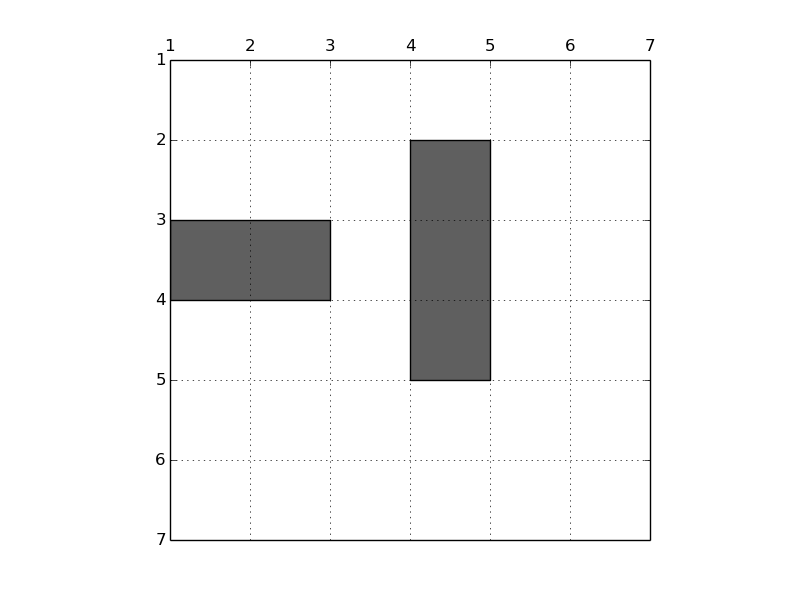
\includegraphics[width=0.4\textwidth]{images/busy.PNG}
  \caption{Posizioni occupate al tempo 0}
  \label{fig:}
\end{figure}



\subsection{Posizioni libere}
A questo punto si definiscono \mint{prolog}|not_free(T,X,Y)| e \mint{prolog}|free(T,X,Y)| che indicano rispettivamente le posizioni della griglia che sono \emph{\textbf{non libere}} e quelle che sono \emph{\textbf{libere}}; in questo modo viene gestita la griglia e le singole posizioni, tralasciando le auto. \\

\noindent
La regola \mint{prolog}|not_free| serve per essere negata nella \mint{prolog}|free| per ottenere la lista di tutte le posizioni libere:
\begin{figure}[H]
\centering
\begin{minted}{prolog}
not_free(T,X,Y) :- time(T), T<l, 
                   grid(X,Y), car(C,_,_), busy(T,C,X,Y).

free(T, X, Y) :- time(T), T<l, 
                 grid(X,Y), car(C,_,_), 
                 not not_free(T,X,Y).
\end{minted}
\label{code:free}
\end{figure}

\noindent
\\Graficamente si ottiene una griglia dove in verde sono rappresentate tutte le posizioni libere.
\begin{figure}[H]
  \centering
  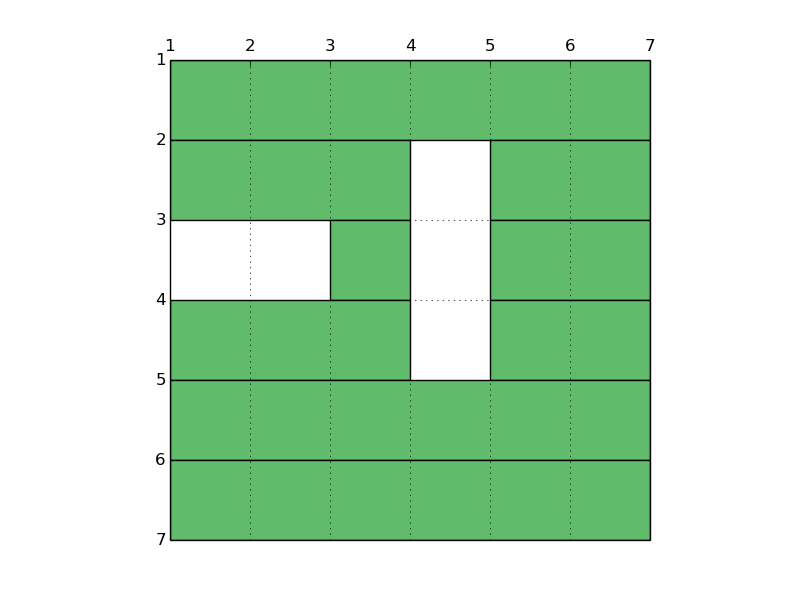
\includegraphics[width=0.4\textwidth]{images/free.PNG}
  \caption{Posizioni libere al tempo 0}
  \label{fig:}
\end{figure}



\subsection{Mosse eseguibili}
Le \emph{\textbf{mosse eseguibili}} sono descritte dalle regole \mint{prolog}|executable|: la testa della regola contiene, oltre che il tempo e il nome dell'auto, la mossa, le coordinate $X$ e le coordinate $Y$, in base al tipo di movimento che l'auto può fare. \\

\noindent % Il movimento rappresentato in basso è il movimento a destra: 
Un auto orizzontale per spostarsi a destra deve lavorare solamente sulle coordinate $Y$ dato che la riga rimane sempre la stessa. La posizione d'interesse si trova a $Y+N$ ed è quella che deve essere libera. \\ %\footnote{Ricordiamo che la posizione dell'auto rappresenta la coppia $(X,Y)$ più piccola}

\noindent
Per eseguire questa mossa è necessario che al tempo $T$ l'auto si trovi in $(X,Y)$.
%La variabile $N$ rappresenta la lunghezza dell'auto e devono essere generate $N$ celle
Un ragionamento equivalente allo spostamento verso destra vale per quello verso il basso di un auto verticale.

\begin{figure}[H]
\centering
\begin{minted}{prolog}
executable(T, C, right, X, Y+1) :- time(T), grid(X,Y+N), 
                                   car(C, N, h), free(T, X, Y+N), 
                                   position(T, C, X, Y).
\end{minted}
\label{code:executable_right}
\end{figure}


\noindent
Lo spostamento verso sinistra e verso l'alto invece, sono leggermente differenti. In particolare la differenza sostanziale riguarda la \mint{prolog}|free|, poichè la posizione che deve essere libera è proprio quella immediatamente a sinistra (o in alto) con ordinata $Y-1$ (o $X-1$).

\begin{figure}[H]
\centering
\begin{minted}{prolog}
executable(T, C, left,  X, Y-1) :- time(T), grid(X,Y-1), 
                                   car(C, N, h), free(T, X, Y-1), 
                                   position(T, C, X, Y).
\end{minted}
\end{figure}


\noindent
Nel nostro caso di esempio, il predicato \mint{prolog}|executable| genera le mosse mostrate in figura \ref{fig:mosse_exec}.

\begin{figure}[H]
     \centering
     \begin{subfigure}[b]{0.3\textwidth}
         \centering
         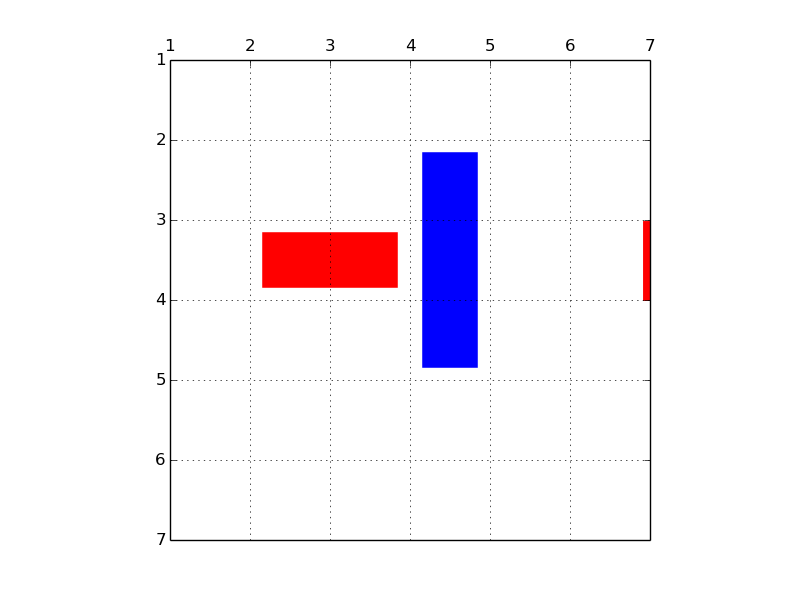
\includegraphics[width=\textwidth]{images/r_right.png}
         \caption{Mossa a destra di r}
     \end{subfigure}
     \hfill
     \begin{subfigure}[b]{0.3\textwidth}
         \centering
         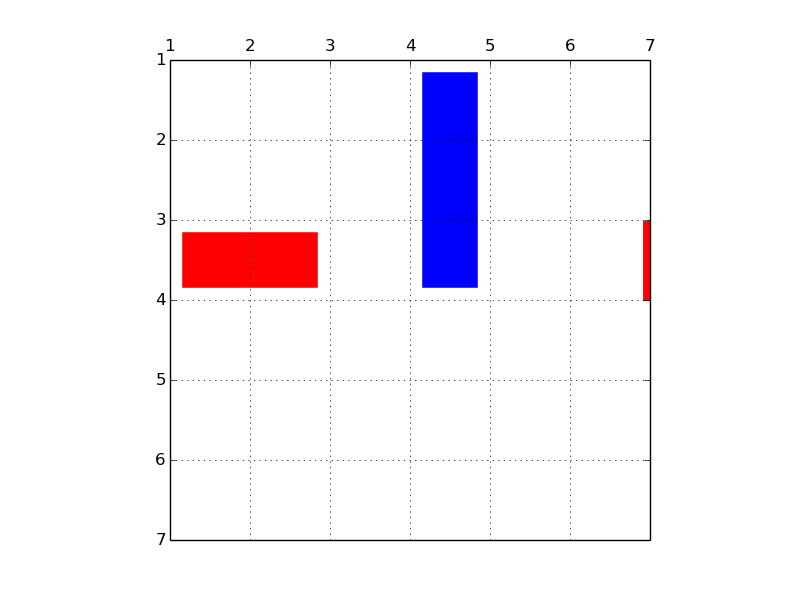
\includegraphics[width=\textwidth]{images/b_up.png}
         \caption{Mossa in alto di b}
     \end{subfigure}
     \hfill
     \begin{subfigure}[b]{0.3\textwidth}
         \centering
         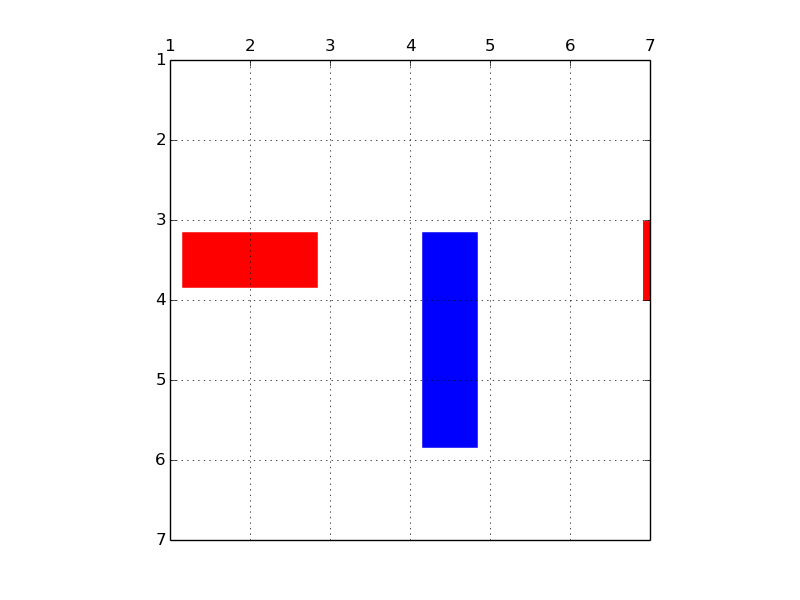
\includegraphics[width=\textwidth]{images/b_down.png}
         \caption{Mossa in basso di b}
     \end{subfigure}
        \caption{Mosse eseguibili al tempo 0}
        \label{fig:mosse_exec}
\end{figure}







\subsection{Scelta della mossa}
A questo punto si prosegue scegliendo una ed una sola mossa eseguibile, a patto che il tempo sia ancora valido:

\begin{figure}[H]
\centering
\begin{minted}{prolog}
1{move(T, C, MOV) : car(C,N,_), executable(T,C,MOV,X,Y)}1 :- time(T), T<l.
\end{minted}
\end{figure}



\subsection{Aggiornamento posizioni}
L'ultimo punto da sviluppare è l'\emph{\textbf{aggiornamento delle posizioni}} al nuovo tempo. È necessario fare una distinzione tra le posizioni delle auto statiche, ovvero quelle che non effettuano nessuna mossa, dalla posizione dell'unica auto che si sposta. \\

\noindent
Supponendo di aver effettuato una mossa al tempo 0 come quella raffigurata, si devono aggiornare le posizioni al tempo 1 di tutte le auto.
\begin{figure}[H]
  \centering
  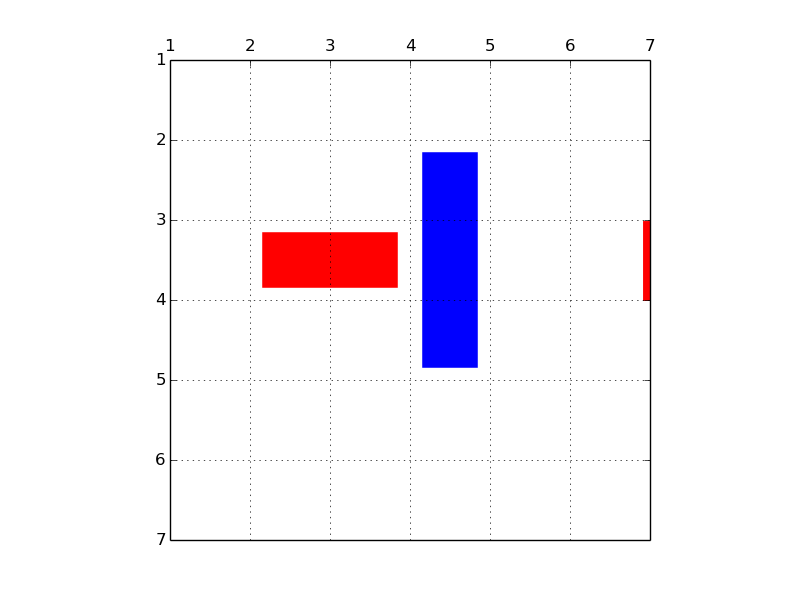
\includegraphics[width=0.4\textwidth]{images/r_right.PNG}
  \caption{Mossa eseguita al tempo 0 e nuove posizioni al tempo 1}
  \label{fig:}
\end{figure}

\noindent
Eseguendo lo spostamento a destra, la nuova posizione $(X,Y)$ al tempo $T$ è dato se, nel tempo precedente, l'auto era di una posizione a sinistra e la mossa che è stata effettuata al tempo precedente era lo spostamento di quell'auto verso destra. \\

\noindent
I casi \emph{left}, \emph{up} e \emph{down} sono equivalenti.

\begin{figure}[H]
\centering
\begin{minted}{prolog}
position(T,C,X,Y) :- moveTo(right), time(T), time(T-1), T<=l, 
                     grid(X,Y-1), position(T-1,C,X,Y-1), car(C,_,h), 
                     move(T-1,C,right).\end{minted}
\end{figure}

\noindent
\\Per le auto che non hanno effettuato nessun movimento è indispensabile mantenere nel nuovo tempo le stesse posizioni che occupavano nel tempo precedente. È stato sufficiente negare il predicato \mint{prolog}|move| nel tempo precedente per avere la certezza che l'auto non si è mossa dalla posizione che occupava.

\begin{figure}[H]
\centering
\begin{minted}{prolog}
position(T,C,X,Y) :- time(T), time(T-1), T<l, 
                     position(T-1,C,X,Y), car(C,_,_), 
                     not move(T-1, C, _).
\end{minted}
\end{figure}



\subsection{Goal}
Definite le regole per generare le posizioni libere o occupate, le mosse possibili e la mossa da eseguire, si procede definendo il \emph{goal}: l'auto rossa deve giungere alla fine della sua riga ed essendo lunga 2, la posizione finale deve essere $(3,5)$. Infatti:

\begin{figure}[H]
\centering
\begin{minted}{prolog}
goal(T) :- time(T), T<l, position(T,r,3,5).
:- not goal(_).
\end{minted}
\end{figure}









\newpage
\section{Ottimizzazioni}

\subsection{Ottimizzazioni sul codice}
Prendendo in esempio la configurazione 2 (file \emph{configuration/sample02.lp}) ed analizzando le varie statistiche del grounder tramite il comando:
\begin{figure}[H]
\centering
\begin{minted}{shell}
gringo rush_hour.lp configuration/sample02.lp -c l=40 | clasp --stat
\end{minted}
\end{figure}

\noindent
Si ottengono le seguenti informazioni (le più rilevanti):
\begin{figure}[H]
\centering
\begin{verbatim}
    Time         : 7.954s (Solving: 7.79s 1st Model: 4.76s Unsat: 3.02s)
    CPU Time     : 7.815s

    Choices      : 237130  
    Conflicts    : 71504    (Analyzed: 71503)
    Restarts     : 227      (Average: 314.99 Last: 237)
\end{verbatim}
\end{figure}

\noindent
Abbiamo un numero elevato di scelte, di conflitti e di restart. Per limitare e cercare di diminuire il più possibile questi dati ci si è incentrati nel modificare alcune regole, soprattutto le \mint{prolog}|position|: la regola che ha un impatto maggiore è quella che ricalcola le posizioni delle auto che non effettuano nessuna mossa:

\begin{figure}[H]
\centering
\begin{minted}{prolog}
position(T,C,X,Y) :- time(T), time(T-1), T<l, 
                     position(T-1,C,X,Y), car(C,_,_), 
                     not move(T-1, C, _).
\end{minted}
\end{figure}

\noindent
\\La variabile \emph{dummy} $\_$ aumenta il numero di atomi e di regole. La decisione presa corrisponde a sostituire queste variabili anonime con quello che davvero ci si aspetta di avere. In basso è possibile vedere la regola modificata.

\begin{figure}[H]
\centering
\begin{minted}{prolog}
position(T,C,X,Y) :- time(T), time(T-1), T<l, 
                     position(T-1,C,X,Y), car(C,N,O), dim(N), orientation(O), 
                     not move(T-1, C, right), not move(T-1, C, left), 
                     not move(T-1, C, up), not move(T-1, C, down).
\end{minted}
\label{code:new_position_v2}
\end{figure}

\noindent
\\In particolare a \mint{prolog}|car| sono state aggiunte la dimensione dell'auto (inserita all'inizio del programma con il fatto \mint{prolog}|dim(2;3).|) e il suo orientamento. \\
Anche la \mint{prolog}|not move| è stata espansa e scritta in modo esplicito con tutti i 4 movimenti che un auto (a prescindere che sia orizzontale o verticale) non può fare per poter essere considerata "ferma" ed è proprio questa modifica che ha portato a risultati migliori. \\

\noindent
Sono state fatte ulteriori piccole modifiche nei corpi delle varie funzioni per essere più stringenti e per limitare ulteriormente le scelte e i conflitti che il programma ha. \\

\noindent
Infatti, analizzando nuovamente il grounding notiamo un netto miglioramento delle performance:
\begin{figure}[H]
\centering
\begin{verbatim}
    Time         : 4.124s (Solving: 3.95s 1st Model: 2.91s Unsat: 1.04s)
    CPU Time     : 4.051s

    Choices      : 116361  
    Conflicts    : 48310    (Analyzed: 48309)
    Restarts     : 171      (Average: 282.51 Last: 39)
\end{verbatim}
\end{figure}















% \begin{figure}[H]
% \centering
% \begin{BVerbatim}
% Time         : 300.414s (Solving: 299.79s 1st Model: 299.77s Unsat: 0.00s)
% CPU Time     : 1011.184s
% Threads      : 4        (Winner: 0)
% \end{BVerbatim}
% \end{figure}



% \noindent
% NON IL GROUJDING!!!!!	
% Per limitare il grounding si è ragionato sulle mosse eseguibili: in una versione precedente, si controllava che un certo range di $X$ o $Y$ facessero parte della griglia per determinare se era possibile o meno spostarsi, come nello snippet sottostante. 
% \begin{figure}[H]
% \centering
% \begin{minted}{prolog}
% executable(T, C, right, X, Y+1) :- time(T), grid(X,Y+1..Y+N), 
%                                    car(C, N, h), free(T, X, Y+N), 
%                                    position(T, C, X, Y).
% \end{minted}
% \end{figure}



% \noindent
% La cella che effettivamente aveva importanza e senso controllare (\mint{prolog}|grid|) era quella successiva all'auto in questione, quella di coordinata $(X,Y+N)$. Apportate queste modifiche, che sono evidenziate in \ref{code:executable_right}, ed eseguendo la nuova versione del codice, il miglioramento ottenuto è il seguente:
% \begin{figure}[H]
% \centering
% \begin{BVerbatim}
% Time         : 201.249s (Solving: 200.61s 1st Model: 200.60s Unsat: 0.00s)
% CPU Time     : 785.106s
% Threads      : 4        (Winner: 0)
% \end{BVerbatim}
% \end{figure}


% \noindent
% Provando con situazioni più complicate, il guadagno di tempo si aggira sempre intorno ai 100/200 secondi. I predicati \mint{prolog}|executable| corrispondono alle mosse che possono essere eseguite ed ampliando la loro cardinalità, il grounder lavora molto di più. \\

% \subsection{Thread}
% sh 1-go sample3.lp 60
% Models       : 1+
% Calls        : 1
% Time         : 9.408s (Solving: 9.11s 1st Model: 9.10s Unsat: 0.00s)
% CPU Time     : 35.962s
% Threads      : 4        (Winner: 3)

% Altra esecuzione con i thread
% Models       : 1+
% Calls        : 1
% Time         : 16.703s (Solving: 16.40s 1st Model: 16.40s Unsat: 0.00s)
% CPU Time     : 64.100s
% Threads      : 4        (Winner: 1)

% Senza thread
% Models       : 1+
% Calls        : 1
% Time         : 29.337s (Solving: 29.05s 1st Model: 29.05s Unsat: 0.00s)
% CPU Time     : 29.107s


\subsection{Multishot}
Dare un tempo massimo di esecuzione per una determinata configurazione non è molto vantaggioso in termini di tempo poichè il goal potrebbe essere soddisfatto in un tempo minore. Si vorrebbe partire dal tempo 0 e, una volta raggiunto il goal minimo, il programma deve terminare.\\

\noindent
La situazione appena descritta rappresenta il cosiddetto \emph{incremental solving}. Con il \emph{multishot} è stato possibile effettuare la ricerca della soluzione di una configurazione in modo incrementale tramite un programma in python e modificando il codice sorgente del risolutore di Rush Hour. \\

\noindent
Sono le direttive \mint{prolog}|#program check(l).| e \mint{prolog}|#program step(l).| che forniscono la variabile tempo al programma. Infatti, le teste delle regole sono cambiate sostituendo la variabile \mint{prolog}|T| con l'atomo \mint{prolog}|l|. \\

\noindent
La nuova testa e il corpo di \mint{prolog}|position| diventa:
\begin{figure}[H]
\centering
\begin{minted}{prolog}
position(l,C,X,Y) :- position(l-1,C,X,Y), car(C,N,O), dim(N), orientation(O), 
                     not move(l-1, C, right), not move(l-1, C, left), 
                     not move(l-1, C, up), not move(l-1, C, down).
\end{minted}
\end{figure}


\noindent
\\Confrontando i tempi di esecuzione tra una versione del programma che utilizza \mint{prolog}|#minimize| con una che utilizza il multishot si ha un notevole guadagno di tempo. Eseguiamo i programmi con i seguenti comandi:
\begin{figure}[H]
\centering
\begin{minted}{shell}
clingo configuration/sample01.lp rush_hour_minimize.lp -c l=40

python3 inc.py configuration/sample01.lp rush_hour_multishot.lp
\end{minted}
\end{figure}
%3.459s
%0.647s

% 5.022s
% 10.224s

% 125.163s
% 41.340s

% ..
% 2492.302s



\noindent
Non è noto a priori quante mosse sono necessarie per giungere al goal: alcune volte il multishot è più lento di una minimize poichè può capitare che il tempo scelto per il programma \mint{shell}|rush_hour_minimize.lp| è proprio quello minimo e l'esecuzione è molto veloce. Questa situazione è capitata analizzando i tempi con la configurazione \mint{shell}|sample02|.

\begin{figure}[H]
  \centering
  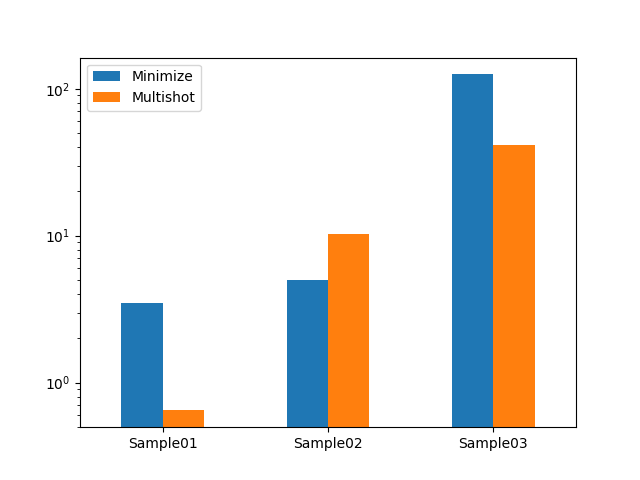
\includegraphics[width=0.6\textwidth]{../images/minimize_vs_multishot.png}
\end{figure}






% \subsection{Confronto con diversi solver}
% ...














\newpage
\section{Implementazione versione 2}
In questa soluzione, per definire il puzzle, vengono usati i predicati:
\begin{itemize}
    \item \mint{prolog}|time/1|: serve a tenere traccia del numero di mosse effettuate in ogni momento;

    \item \mint{prolog}|grid/2|: indica tutte le coordinate della griglia in cui le auto vengono poste;

    \item \mint{prolog}|no/2|: indica se una certa posizione della griglia è invalicabile;

    \item \mint{prolog}|orientation/1|: indica il verso in cui l'auto può essere posta (orizzontale e verticale);

    \item \mint{prolog}|position/6| e \mint{prolog}|position/7|: indicano la posizione di una certa auto in un certo tempo.
\end{itemize}




\subsection{Posizioni}
I predicati \mint{prolog}|position| con il primo argomento posto a zero indicano la posizione dell'auto \mint{prolog}|C| al tempo iniziale. \mint{prolog}|O| indica il verso dell'auto, mentre \mint{prolog}|C1|, \mint{prolog}|C2|, \mint{prolog}|C3| e \mint{prolog}|C4| indicano le coordinate sulla griglia dell'auto. Le coordinate sono dipendenti da \mint{prolog}|O| in questo modo:
\begin{itemize}
    \item Se \mint{prolog}|O| viene sostituito con l'atomo \mint{prolog}|h|, allora \mint{prolog}|C1| rappresenta la coordinata \mint{prolog}|X| dell'auto, mentre \mint{prolog}|C1|, \mint{prolog}|C2| e \mint{prolog}|C3| rappresentano le coordinate \mint{prolog}|Y|;
    \item Se \mint{prolog}|O| viene sostituito con l'atomo \mint{prolog}|v|, allora \mint{prolog}|C1| rappresenta la coordinata \mint{prolog}|Y| dell'auto, mentre \mint{prolog}|C1|, \mint{prolog}|C2| e \mint{prolog}|C3| rappresentano le coordinate \mint{prolog}|X|.
\end{itemize}

\noindent
Usando questo approccio siamo in grado di spostare tutta l'auto in un solo colpo senza dover cercare tutti i predicati che appartengono a un'auto. \\

\noindent
Il problema di questo approccio è che non è parametrizzabile, quindi se ad esempio si volessero aggiungere auto di dimensione 4 è necessario estendere il programma. \\

\noindent
Per questione di comodità, da ora in poi vedremo le regole per le auto di dimensione 2 e orizzontali, ma è intuitivo ricavare le stesse regole per auto di dimensione 3 e poste verticalmente a partire dalle seguenti.

\begin{figure}[H]
\centering
\begin{minted}{prolog}
position(T+1, C, h, C1, C2, C3) :-
    cause(T, move(_, C), position(T+1, C, h, C1, C2, C3)),
    time(T), time(T+1), car(C),
    grid(C1, C2), grid(C1, C3).
\end{minted}
\end{figure}


\noindent
\\ Questa regola \mint{prolog}|position/6| serve ad aggiornare la posizione dell'auto \mint{prolog}|C| al tempo
\mint{prolog}|T+1| se è stata spostata al tempo \mint{prolog}|T|.

\begin{figure}[H]
\centering
\begin{minted}{prolog}
position(T+1, C, h, C1, C2, C3) :-
    not executed(T, move(_, C)),
    position(T, C, h, C1, C2, C3),
    time(T), car(C),
    grid(C1, C2), grid(C1, C3).
\end{minted}
\end{figure}


\noindent
\\Questa regola \mint{prolog}|position/6| corrisponde all'invariante di posizione. Se non è stata compiuta nessuna azione sull'auto \mint{prolog}|C| al tempo \mint{prolog}|T| allora la sua posizione sarà la stessa anche al tempo \mint{prolog}|T+1|.




\subsection{Posizioni libere}
La regola \mint{prolog}|not_free/3| indica che una cella $(X,Y)$ della griglia è occupata al tempo $T$ se c'è un auto che occupa quella posizione al tempo $T$.

\begin{figure}[H]
\centering
\begin{minted}{prolog}
not_free(T, X, Y) :-
    position(T, _, h, X, Y, _).
not_free(T, X, Y) :-
    position(T, _, h, X, _, Y).
\end{minted}
\end{figure}

\noindent
\\La regola \mint{prolog}|free/3| indica che una cella $(X,Y)$ della griglia è libera al tempo $T$.
se non è occupata al tempo T.

\begin{figure}[H]
\centering
\begin{minted}{prolog}
free(T, X, Y) :-
    time(T), grid(X, Y),
    not not_free(T, X, Y).
\end{minted}
\end{figure}



\subsection{Azioni possibili}
La regola \mint{prolog}|action/2| indica che un'auto \mint{prolog}|C| può muoversi a destra nel tempo $T$ se la cella alla sua destra immediata non è occupata da nessun'auto ed è valicabile. Lo stesso ragionamento viene applicato per gli spostamenti verso le altre direzioni.

\begin{figure}[H]
\centering
\begin{minted}{prolog}
action(T, move(right, C)) :-
    car(C), time(T),
    position(T, C, h, X, Y1, Y2),
    free(T, X, Y2+1),
    not no(X, Y2+1),
    grid(X, Y2+1).
\end{minted}
\end{figure}


\subsection{Azione scelta}
La regola \mint{prolog}|executed/2| è quella che effettua l'azione, ovvero tra tutte le azioni generate tramite la regola \mint{prolog}|action/2| ne sceglie una e la esegue.

\begin{figure}[H]
\centering
\begin{minted}{prolog}
1 {executed(T, move(Dir, C)): action(T, move(Dir, C))} 1 :-
    time(T), T < t.
\end{minted}
\end{figure}




\subsection{Cause}
La regola \mint{prolog}|cause/3| è necessario per effettuare l'update della posizione dell'auto \mint{prolog}|C|, spostata a destra di una casella tramite la regola \mint{prolog}|executed/2|. Lo stesso ragionamento viene applicato per gli spostamenti verso le altre direzioni.

\begin{figure}[H]
\centering
\begin{minted}{prolog}
cause(T, move(right, C), position(T+1, C, h, X, Y1+1, Y2+1)) :-
    executed(T, move(right, C)),
    car(C), time(T+1), time(T),
    position(T, C, h, X, Y1, Y2),
    free(T, X, Y2+1),
    not no(X, Y2+1),
    grid(X, Y2+1).
\end{minted}
\end{figure}















\newpage
\section{Risultati}
L'analisi del grounding, con l'aggiunta di auto e con tempi maggiori, è diventata sempre più lunga e complessa. È stato sviluppato un programma in python che si occupa di salvare inizialmente le informazioni riguardo la struttura delle auto, prima di disegnare graficamente le auto nelle posizioni che occupano in un dato tempo. \\

\noindent
I disegni sono stati fatti tramite la libreria \emph{matplotlib}, sono stati salvati e successivamente riuniti in un file gif per poter vedere facilmente la risoluzione del caso scelto e fornito al programma. \\


\subsection{Confronto versioni}
Nell'analisi delle due versioni sviluppate c'è una sostanziale differenza in termini di tempo. La versione più "stringata" (per convenzione la versione 2) e leggermente più complicata da capire a primo impatto, funziona molto meglio ed ha tempi di esecuzione molto più bassi rispetto all'altro programma (versione 1). %, con configurazioni via via sempre più complicate.\\

\begin{figure}[H]
  \centering
  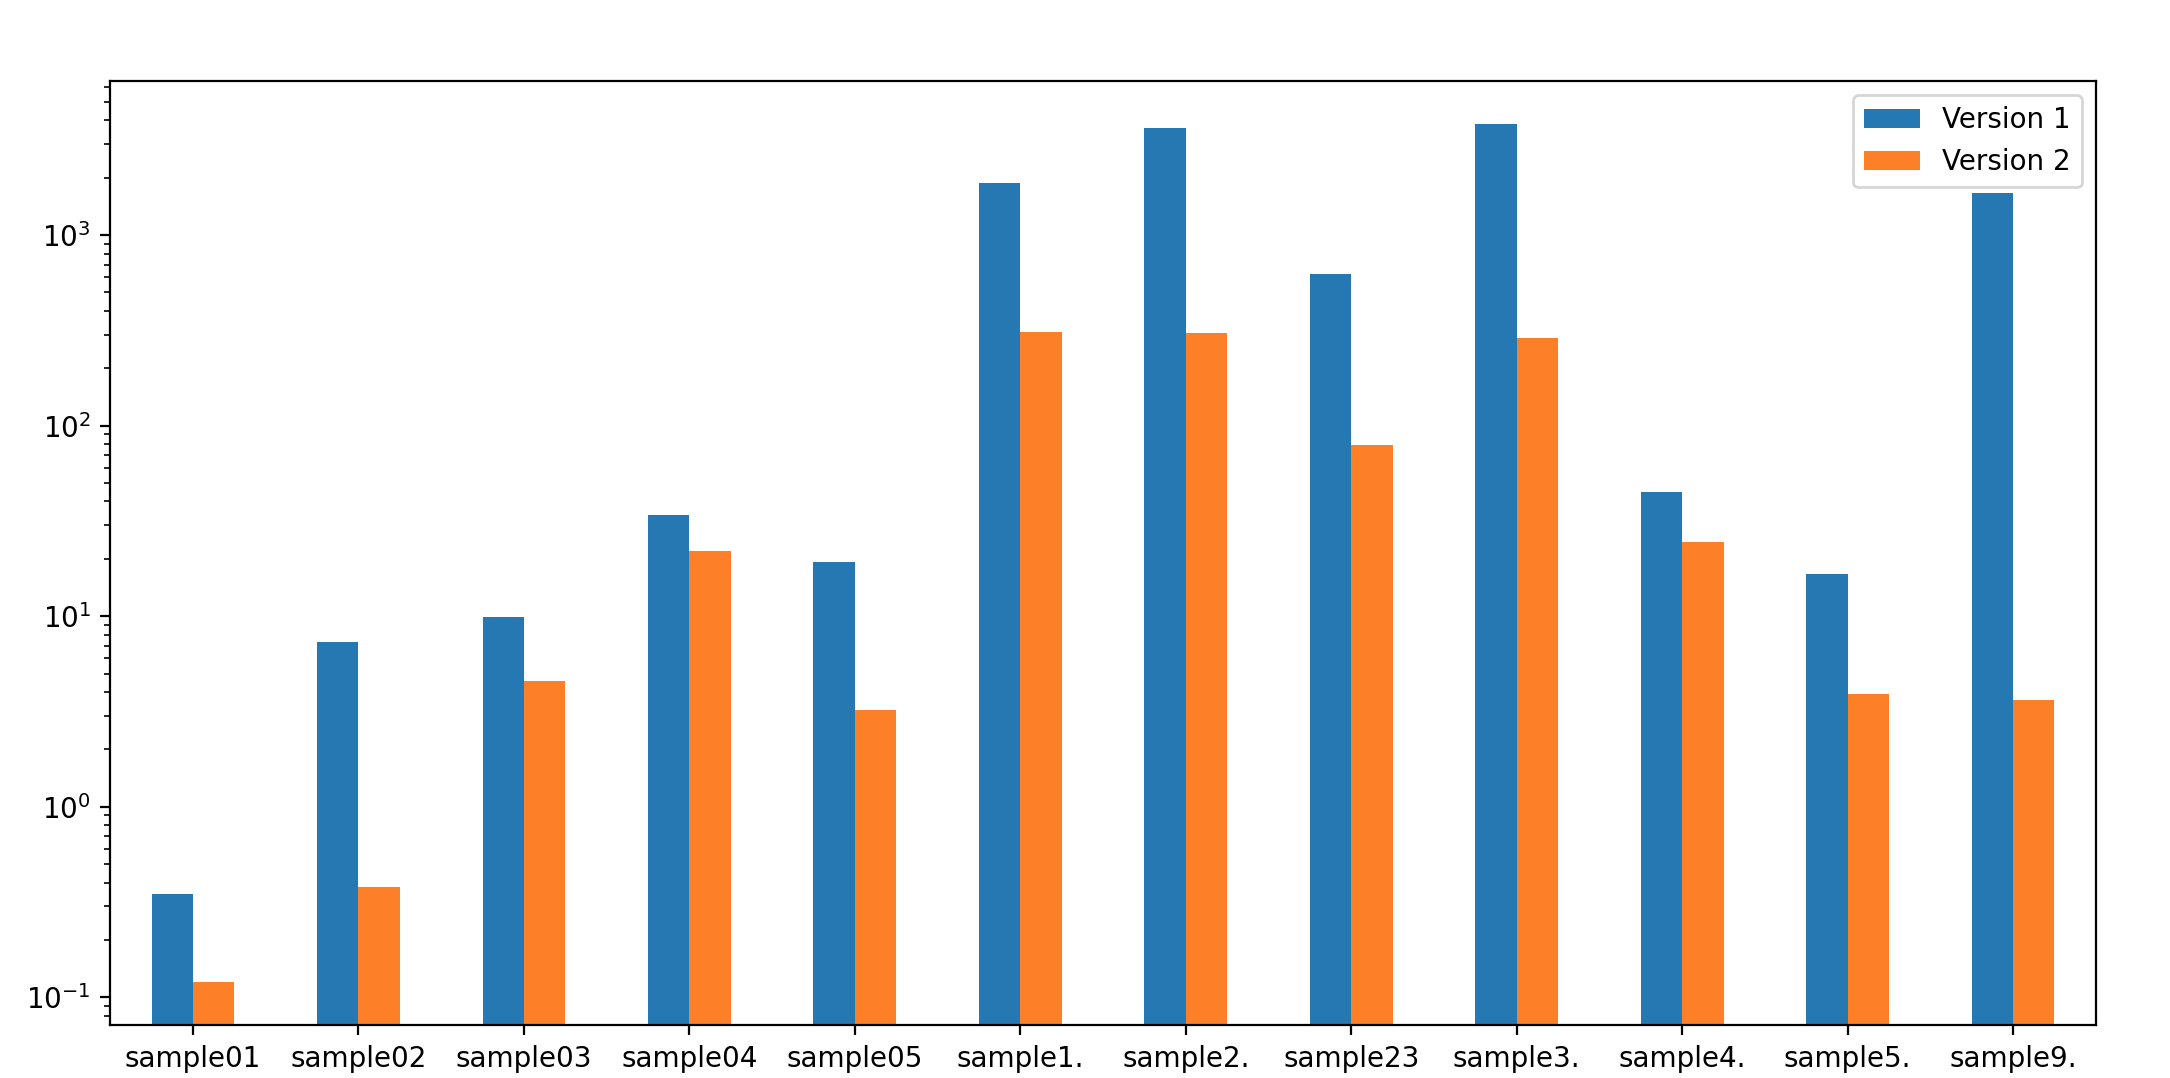
\includegraphics[width=1\textwidth]{../images/stats2.PNG}
  \caption{Confronto dei tempi di esecuzione delle due versioni}
  \label{fig:confronto_tempi}
\end{figure}

\noindent
Per fare il confronto dei tempi mostrato in figura \ref{fig:confronto_tempi}, sono state utilizzate le stesse configurazioni, ovviamente codificate nel modo opportuno e senza multishot, facendo raggiungere il goal nel tempo da noi fissato (evitando quindi la \mint{prolog}|minimize|). \\

% \noindent
% Per essere un po più a conoscenza del motivo di questo divario, abbiamo analizzato le varie statistiche del grounder, tramite il comando \mint{shell}|clasp --stat|, posto in \emph{pipe} dopo l'esecuzione del grounder con \mint{shell}|gringo|. \\

% \noindent
% I risultati (di seguito mostrati nelle righe più interessanti), sono i seguenti: \\
% ...\\
% ...\\
% ...\\


\noindent
Da notare anche come, ad esempio, per creare l'istanza della configurazione \emph{sample02.lp}, il grounding sia diventato di dimensione:


\begin{table}[H]
    \centering
    \begin{tabular}{c|c|c|c|}
    \cline{2-4}
    \textit{\textbf{}}                        & \textit{Numero righe} & \textit{Numero parole} & \textit{Byte} \\ \hline
    \multicolumn{1}{|c|}{\textit{Versione 1}} & 31184                 & 225893                 & 876816       \\ \hline
    \multicolumn{1}{|c|}{\textit{Versione 2}} & 19248                 & 130794                 & 540640       \\ \hline
    \end{tabular}
\end{table}






\end{document}